\documentclass[dvipsnames, usenames]{beamer}

\usetheme{cleancode}
\usepackage[T1]{fontenc}
\usepackage[ansinew]{inputenc}
\usepackage[USenglish]{babel}
\usepackage{amsmath}
\usepackage{mathtools}
\usepackage{stmaryrd}
\usepackage{graphicx}
\usepackage{lmodern}
%\usepackage{tcolorbox}

\usepackage[round, authoryear]{natbib}
\usepackage{subcaption}
\usepackage[export]{adjustbox}

% Graph Picture Packages
\usepackage{tikz}
\usetikzlibrary{positioning}
\usetikzlibrary{calc}

\usepackage{amsthm, amssymb, amsfonts, amsmath, xcolor}
\def\boxitem#1{\setbox0=\vbox{#1}{\centering\makebox[0pt]{%
  \fboxrule=2pt\color{red}\fbox{\hspace{\leftmargini}\color{black}\box0}}\par}}


\usepackage{algorithm,algorithmicx,algpseudocode}
\algnewcommand\algorithmicinput{\textbf{Input:}}
\algnewcommand\INPUT{\item[\algorithmicinput]}
\algnewcommand\algorithmicoutput{\textbf{Output:}}
\algnewcommand\OUTPUT{\item[\algorithmicoutput]}
\algnewcommand\algorithmicidea{\textbf{Idea:}}
\algnewcommand\IDEA{\item[\algorithmicidea]}
\algnewcommand\algorithmicinit{\textbf{Initialize:}}
\algnewcommand\INIT{\item[\algorithmicinit]}

\algnewcommand\algorithmicforeach{\textbf{for each}}
\algdef{S}[FOR]{ForEach}[1]{\algorithmicforeach\ #1\ \algorithmicdo}


\newcommand\Wider[2][3em]{%
\makebox[\linewidth][c]{%
  \begin{minipage}{\dimexpr\textwidth+#1\relax}
  \raggedright#2
  \end{minipage}%
  }%
}

\usepackage{bibentry, bibentry}

% Generates new title page at beginning of each section
\AtBeginSection[]{
  \begin{frame}
  \vfill
  \centering
  \begin{beamercolorbox}[sep=8pt,center,shadow=true,rounded=true]{title}
    \usebeamerfont{title}\insertsectionhead\par%
  \end{beamercolorbox}
  \vfill
  \end{frame}
}
\setbeamertemplate{navigation symbols}{}


\DeclareMathOperator*{\plim}{plim}

\setbeamertemplate{footline}[frame number]
\setbeamertemplate{theorems}[numbered]

\newcommand{\R}{\mathbb{R}}
\newcommand{\N}{\ensuremath{\mathcal{N}}}


\pgfdeclareimage[width=0.7\paperwidth]{mybackground}{../figures/report/datasets}
%
%\setbeamertemplate{title page}{
%
%        \begin{picture}(0,0)
%
%            \put(-30,-100){%
%                \pgfuseimage{mybackground}
%            }
%
%            \put(0,-110.7){%
%                \begin{minipage}[b][45mm][t]{226mm}
%                    \usebeamerfont{title}{\inserttitle\par}
%                    	\usebeamerfont{author}{\insertauthor\par}
%                \end{minipage}
%            }
%
%            \end{picture}
%
%    }


\begin{document}

%------------------------------------------------------------------------------%
% Setup TikzStyle

\tikzstyle{block} = [rectangle, draw, 
    text width=5em, text centered, rounded corners, minimum height=1.5em]
    
\tikzstyle{line} = [draw, -latex]

\title{Biologically Plausible Deep Learning: \\ A Critical Review}
\subtitle{}

\author{\texorpdfstring{Robert Tjarko Lange\thanks{\url{https://github.com/RobertTLange/Bio-Plausible-DeepLearning}}
						\newline\url{rtl17@ic.ac.uk}
						\newline\url{www.rob-lange.com}
	}
	{Author}}


\institute{Einstein Center for Neurosciences Berlin}
\date{\today}


%------------------------------------------------------------------------------%

\begin{frame}[noframenumbering]

\titlepage
\begin{picture}(0,0)
\put(+25,+0){\pgfuseimage{mybackground}}
\end{picture}
\end{frame}

%------------------------------------------------------------------------------%
\begin{frame}{Motivation}
\vspace{-0.5cm}

\end{frame}

%------------------------------------------------------------------------------%
\begin{frame}{Literature Review}
\vspace{-0.5cm}

\begin{figure}[H]
	\centering
	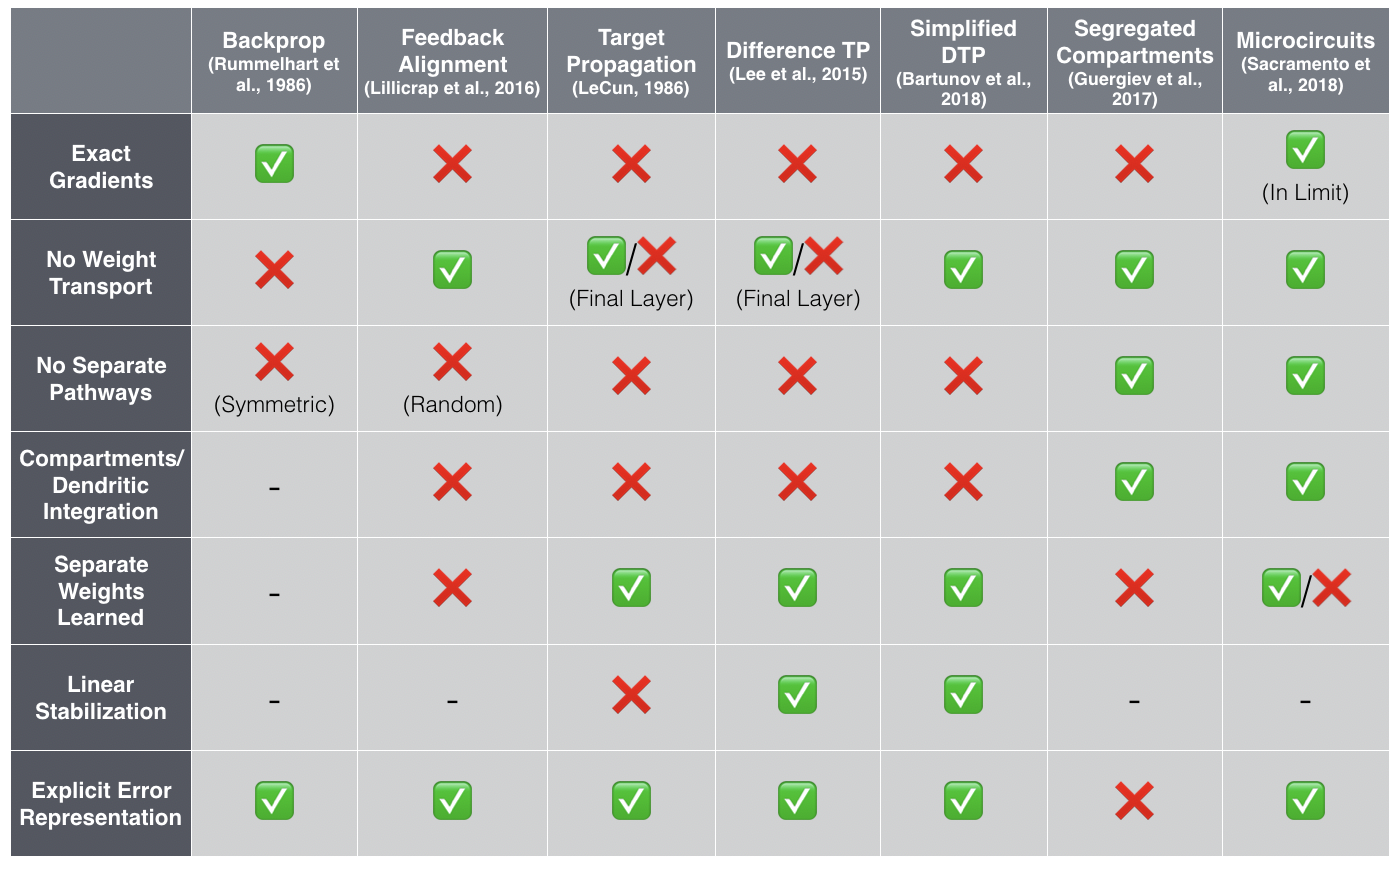
\includegraphics[width=\textwidth]{../figures/report/lit_rev}
\end{figure}

\end{frame}

%------------------------------------------------------------------------------%
\begin{frame}{\citet{guerguiev2017}}
\vspace{-0.5cm}



\end{frame}


%------------------------------------------------------------------------------%

\begin{frame}{What's next?}
\vspace{-0.5cm}


\end{frame}



%------------------------------------------------------------------------------%

\begin{frame}[allowframebreaks, noframenumbering]{References}
   \begin{tiny}
   \setbeamertemplate{bibliography item}[text]
   \bibliographystyle{authordate1}
   \bibliography{main.bib}
   \end{tiny}
\end{frame}



%------------------------------------------------------------------------------%
\appendix


\begin{frame}

\end{frame}

%------------------------------------------------------------------------------%



\end{document} 